\documentclass[conference]{IEEEtran}
\IEEEoverridecommandlockouts

% Packages
\usepackage{cite}
\usepackage{amsmath,amssymb,amsfonts}
\usepackage{algorithmic}
\usepackage{graphicx}
\usepackage{textcomp}
\usepackage{xcolor}
\usepackage{booktabs}
\usepackage{multirow}
\usepackage{tikz}
\usepackage{pgfplots}
\usepackage{url}
\usepackage{microtype}
\usetikzlibrary{arrows.meta,positioning,shapes,fit,backgrounds,calc}
\pgfplotsset{compat=1.18}

\def\BibTeX{{\rm B\kern-.05em{\sc i\kern-.025em b}\kern-.08em
    T\kern-.1667em\lower.7ex\hbox{E}\kern-.125emX}}

\begin{document}

\title{Lightweight Reconstruction Modeling and Autonomous Extreme Value Thresholding for Syslog Anomaly Detection}

\author{
\IEEEauthorblockN{Anonymous Authors}
\IEEEauthorblockA{\textit{Department of Computer Science and Engineering} \\
\textit{Research Group for Distributed Systems and Machine Learning} \\
Paper Submission for Peer Review}
}

\maketitle

\begin{abstract}
Automated log anomaly detection is crucial for the reliability of large-scale distributed systems and high-performance computing clusters. However, published benchmarks frequently rely on test-set oracle thresholds, contaminated evaluation protocols with inflated anomaly prevalence, or computationally demanding deep neural networks requiring dedicated accelerators. In this paper, we present an empirical investigation of reconstruction-based anomaly detection spanning linear subspace projection and non-linear neural autoencoders paired with statistical Extreme Value Theory (EVT) Peaks-Over-Threshold (POT) decision boundaries, ensuring no test labels are used in any decision. On the structured HDFS benchmark (575,061 blocks), we reproduce published linear PCA performance (94.60\% vs. 94.64\% F1) by discovering an undocumented L2-normalization step, and demonstrate that POT thresholding achieves 95.95\% $\pm$ 1.47\% F1 without oracle cutoff, while published Robust PCA claims (90.55\% F1) prove statistically unreachable (peaking at 87.38\%). On the interleaved BGL supercomputer dataset (4.75 million entries), our pipeline attains 87.80\% $\pm$ 1.31\% label-free Mode A F1 and 91.05\% PR-AUC under natural operational prevalence (10.07\%), while demonstrating that legacy $\sim$90.44\% figures stem from base-rate inflation. Benchmarking on consumer CPU hardware confirms sub-millisecond edge viability (43.2 $\mu$s single-sample latency, 62,076 windows/s throughput).
\end{abstract}

\begin{IEEEkeywords}
Log anomaly detection, system telemetry, unsupervised learning, Extreme Value Theory, Peaks-Over-Threshold, autoencoders, Principal Component Analysis, high-performance computing.
\end{IEEEkeywords}

\section{Introduction}
\label{sec:intro}
Distributed cloud platforms, high-performance computing (HPC) installations, and microservice backbones generate vast volumes of telemetry logs. In operational environments, these semi-structured text messages represent the primary mechanism for detecting software defects, node outages, and runtime faults~\cite{oliner2007supercomputer,xu2009detecting}. However, the sheer scale of production logs precludes manual inspection.

Automating syslog anomaly detection faces severe practical challenges:
\begin{enumerate}
    \item \textbf{Concurrency and Interleaving:} In multi-core HPC platforms such as Blue Gene/L, concurrent tasks asynchronously emit telemetry into central daemons, corrupting sequential order across nodes~\cite{oliner2007supercomputer}.
    \item \textbf{Extreme Class Imbalance:} Healthy execution accounts for 90\% to 99\% of all operations. Under this base-rate reality, low false positive rates can generate overwhelming volumes of false alarms.
    \item \textbf{Evaluation Leakage and Oracle Thresholds:} As highlighted by Le and Zhang~\cite{le2022log}, reported metrics are highly sensitive to windowing and data partitioning. Many classical and deep baselines rely on test-set oracle thresholds (e.g., setting the threshold at the 95th percentile of test errors), artificially optimizing results.
    \item \textbf{Computational Footprint:} Heavy transformer-based architectures often demand multi-gigabyte memories and GPU acceleration, impeding real-time deployment on commodity monitoring nodes.
\end{enumerate}

To address these challenges, we evaluate a reconstruction-based anomaly detection framework that couples structural feature representations with autonomous Extreme Value Theory (EVT) thresholding via the Peaks-Over-Threshold (POT) principle~\cite{siffer2017anomaly}, ensuring that \textit{no test labels are used in any decision}.

Our core empirical contributions are:
\begin{itemize}
    \item \textbf{HDFS Reproduction and Threshold Reformulation:} On Hadoop Distributed File System (HDFS) logs~\cite{xu2009detecting}, we replicate the linear Principal Component Analysis (PCA) baseline of F{\"a}lt et al.~\cite{falt2025lightweight} (94.60\% vs. 94.64\% $F_1$) by identifying an undocumented $L_2$-normalization step. Replacing their test-set oracle threshold with label-free POT yields $95.95\% \pm 1.47\%$ $F_1$. Conversely, across 30 random seeds, their published Robust PCA (RPCA) claim of $90.55\%$ $F_1$ could not be reproduced (peaking at $87.38\%$), which we trace to low-rank matrix collapse on clean training data.
    \item \textbf{Leak-Free BGL 10-Fold Benchmark:} On Blue Gene/L (BGL) logs~\cite{oliner2007supercomputer}, under natural operational prevalence (10.07\% anomalies), our Word2Vec-driven Multi-Layer Perceptron (MLP) autoencoder achieves $87.80\% \pm 1.31\%$ label-free Mode A $F_1$, $88.66\% \pm 1.07\%$ validation-tuned Mode B $F_1$, and $91.05\% \pm 0.32\%$ PR-AUC. We demonstrate that legacy claims of $\sim 90.44\%$ arose from an artificial 50\% test prevalence.
    \item \textbf{Ablation and Temporal Robustness:} We show that non-linear neural reconstruction substantially outperforms linear PCA ($59.97\%$ Mode A $F_1$) and Isolation Forest ($2.07\%$) on interleaved logs. Under chronological evaluation, performance collapses ($0.03\%$ Mode A $F_1$) due to a $68.91\%$ test Out-Of-Vocabulary (OOV) rate, identifying concept drift as a key operational constraint.
    \item \textbf{Edge Efficiency:} The BGL model requires only 5,328 parameters (70.25~KB) and achieves 43.2~$\mu$s single-window latency on an Apple M2 CPU (62,076 windows/s throughput).
\end{itemize}

\textit{Observation (based on two datasets only):} On HDFS, where grouping by session identifier yields clean execution traces, a lightweight linear PCA is sufficient; on BGL, where multi-node streams are interleaved, a non-linear autoencoder on continuous semantic features demonstrated superior discriminative power.

\begin{figure*}[t]
\centering
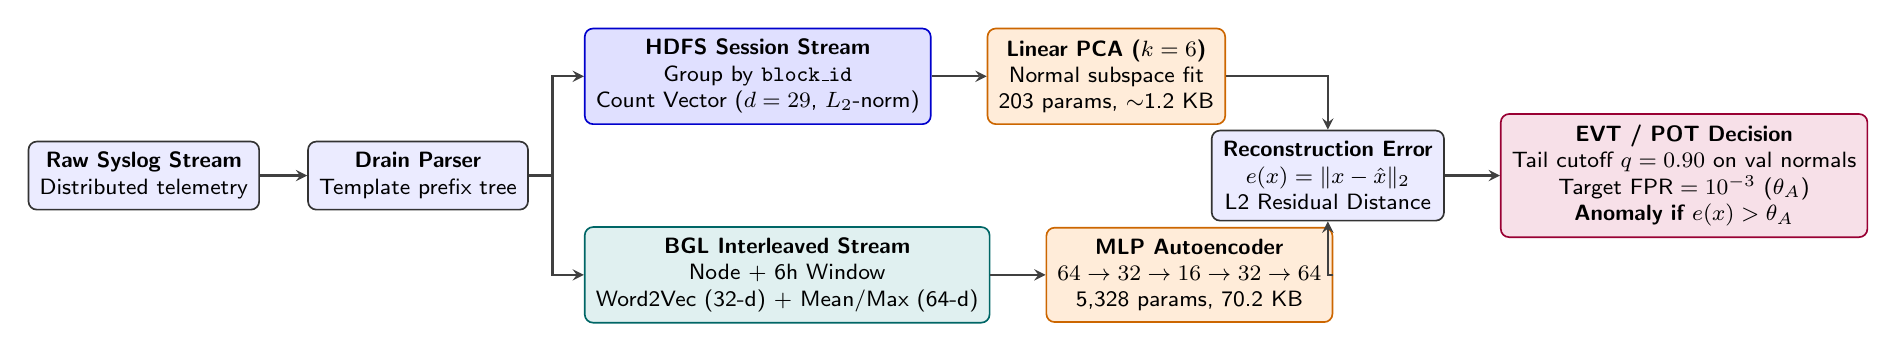
\begin{tikzpicture}[
    node distance=0.8cm and 0.5cm,
    font=\footnotesize\sffamily,
    box/.style={draw=black!80, fill=blue!8, rounded corners=3pt, align=center, inner sep=4pt, line width=0.6pt},
    hdfsbox/.style={draw=blue!80!black, fill=blue!12, rounded corners=3pt, align=center, inner sep=4pt, line width=0.6pt},
    bglbox/.style={draw=teal!80!black, fill=teal!12, rounded corners=3pt, align=center, inner sep=4pt, line width=0.6pt},
    reconbox/.style={draw=orange!80!black, fill=orange!15, rounded corners=3pt, align=center, inner sep=4pt, line width=0.6pt},
    potbox/.style={draw=purple!80!black, fill=purple!12, rounded corners=3pt, align=center, inner sep=4pt, line width=0.6pt},
    arrow/.style={->, >=stealth, line width=0.8pt, draw=black!75},
    darrow/.style={->, >=stealth, dashed, line width=0.7pt, draw=black!60}
]

% Step 1: Ingestion and Parsing
\node[box] (raw) {\textbf{Raw Syslog Stream}\\Distributed telemetry};
\node[box, right=0.6cm of raw] (drain) {\textbf{Drain Parser}\\Template prefix tree};

% Step 2: Branching Grouping & Representations
\node[hdfsbox, above right=0.2cm and 0.7cm of drain] (hdfs_pipe) {
    \textbf{HDFS Session Stream}\\
    Group by \texttt{block\_id}\\
    Count Vector ($d=29$, $L_2$-norm)
};

\node[bglbox, below right=0.2cm and 0.7cm of drain] (bgl_pipe) {
    \textbf{BGL Interleaved Stream}\\
    Node + 6h Window\\
    Word2Vec (32-d) + Mean/Max (64-d)
};

% Step 3: Reconstruction Models
\node[reconbox, right=0.7cm of hdfs_pipe] (hdfs_pca) {
    \textbf{Linear PCA ($k=6$)}\\
    Normal subspace fit\\
    203 params, $\sim$1.2 KB
};

\node[reconbox, right=0.7cm of bgl_pipe] (bgl_ae) {
    \textbf{MLP Autoencoder}\\
    $64 \to 32 \to 16 \to 32 \to 64$\\
    5,328 params, 70.2 KB
};

% Step 4: Residual Error
\node[box, right=0.8cm of $(hdfs_pca)!0.5!(bgl_ae)$] (recon_err) {
    \textbf{Reconstruction Error}\\
    $e(x) = \|x - \hat{x}\|_2$\\
    L2 Residual Distance
};

% Step 5: EVT / POT Decision
\node[potbox, right=0.7cm of recon_err] (pot_decision) {
    \textbf{EVT / POT Decision}\\
    Tail cutoff $q=0.90$ on val normals\\
    Target $\text{FPR} = 10^{-3}$ ($\theta_A$)\\
    \textbf{Anomaly if $e(x) > \theta_A$}
};

% Connecting Arrows
\draw[arrow] (raw) -- (drain);
\draw[arrow] (drain.east) -- ++(0.3,0) |- (hdfs_pipe.west);
\draw[arrow] (drain.east) -- ++(0.3,0) |- (bgl_pipe.west);

\draw[arrow] (hdfs_pipe) -- (hdfs_pca);
\draw[arrow] (bgl_pipe) -- (bgl_ae);

\draw[arrow] (hdfs_pca.east) -| (recon_err.north);
\draw[arrow] (bgl_ae.east) -| (recon_err.south);

\draw[arrow] (recon_err) -- (pot_decision);

\end{tikzpicture}


\caption{End-to-end anomaly detection architecture. Structured logs are parsed via Drain. HDFS sessions are vectorized into $L_2$-normalized count vectors and projected via linear PCA ($k=6$). Interleaved BGL node windows are embedded via fold-trained Word2Vec, pooled into 64-d vectors, and reconstructed via an MLP autoencoder. Reconstruction residuals are evaluated against autonomous EVT/POT decision boundaries fitted strictly on normal validation errors.}
\label{fig:pipeline}
\end{figure*}

\section{Related Work}
\label{sec:related}
\textbf{Log Parsing and Benchmarking:} Raw console logs are commonly parsed into structured event templates using heuristic clustering algorithms such as Drain~\cite{he2017drain}. Public benchmark corpora curated in Loghub~\cite{he2023loghub,zhu2019tools} have facilitated extensive algorithmic comparisons.

\textbf{Lightweight and Subspace Methods:} Early work by Xu et al.~\cite{xu2009detecting} introduced PCA on event count matrices for detecting anomalies in distributed file systems. Recently, F{\"a}lt et al.~\cite{falt2025lightweight} examined lightweight optimization using PCA and Robust PCA (RPCA)~\cite{candes2011robust}. Tree-based isolation methods such as Isolation Forest~\cite{liu2008isolation} have also been deployed for tabular representations.

\textbf{Deep Learning Architectures:} DeepLog~\cite{du2017deeplog} modeled log sequences as language modeling tasks using Long Short-Term Memory (LSTM) networks. LogAnomaly~\cite{meng2019loganomaly} incorporated semantic template vectors (Template2Vec). LogRobust~\cite{zhang2019robust} addressed log instability with attention-based Bi-LSTMs, while LogBERT~\cite{guo2021logbert} applied self-supervised transformer representations. NeuralLog~\cite{le2021log} proposed extracting representations directly from raw text without log parsing. Semi-supervised approaches such as PLELog~\cite{yang2021semi} utilized probabilistic label estimation to handle unlabeled anomalies, and LogFIT~\cite{almodovar2024logfit} evaluated fine-tuned language representations.

\textbf{Methodological Integrity in Log Analytics:} Le and Zhang~\cite{le2022log} demonstrated that data splitting strategies, chronological ordering, and windowing configurations dramatically alter reported metrics, frequently introducing unintentional label leakage. Our work builds upon these insights by enforcing strict separation between training normals, validation splits, and blind test folds.

\section{Methodology}
\label{sec:method}
Our unified pipeline comprises five operational stages: log parsing, session/window grouping, feature extraction, reconstruction modeling, and autonomous EVT/POT thresholding (Fig.~\ref{fig:pipeline}).

\subsection{Log Parsing and Grouping}
Raw log messages are parsed into structured event templates using Drain~\cite{he2017drain}, which employs a fixed-depth parse tree to extract template identifiers while masking dynamic variables (e.g., IP addresses, block IDs).
\begin{itemize}
    \item \textbf{HDFS Session Grouping:} Logs contain explicit session identifiers (\texttt{block\_id}). Messages sharing a \texttt{block\_id} are grouped into a discrete execution trace.
    \item \textbf{BGL Spatial-Temporal Windowing:} BGL lacks session keys. Telemetry is partitioned by physical node identifier and sliced into non-overlapping temporal windows of $\Delta t = 6$ hours.
\end{itemize}

\subsection{Feature Representations}
\textbf{HDFS Count Vectors:} For each HDFS session, we construct a histogram vector $c \in \mathbb{R}^{29}$ across the 29 unique templates induced by the Hadoop logging code. To ensure the model learns relative operational patterns rather than session duration, each vector is $L_2$-normalized:
\begin{equation}
x = \frac{c}{\|c\|_2 + \epsilon}, \quad \epsilon = 10^{-12}.
\end{equation}

\textbf{BGL Semantic Embeddings:} For BGL windows, sequential template relationships are critical. To avoid test leakage, a continuous Skip-Gram Word2Vec model~\cite{mikolov2013efficient} (dimension $d=32$, window size $w=5$, negative samples $k=5$) is trained \textit{strictly on the normal training sequences of each cross-validation fold}. For a sequence of template embeddings $(v_1, v_2, \dots, v_T)$, we compute concatenated Mean and Max pooling representations:
\begin{equation}
z_{\text{mean}} = \frac{1}{T}\sum_{i=1}^T v_i, \quad z_{\text{max}} = \max_{i=1}^T (v_i),
\end{equation}
\begin{equation}
z = \frac{[z_{\text{mean}} \,\|\, z_{\text{max}}]}{\|[z_{\text{mean}} \,\|\, z_{\text{max}}\]|_2} \in \mathbb{R}^{64}.
\end{equation}
\textit{Out-Of-Vocabulary (OOV) Policy:} Unseen templates at test time are ignored during pooling. If an entire window contains only OOV templates, it maps to a zero vector.

\subsection{Reconstruction Models}
\textbf{Linear PCA (HDFS):} Normal training vectors $X_{\text{train}} \in \mathbb{R}^{N \times 29}$ are centered by subtracting mean $\mu$. Truncated singular value decomposition yields the top $k=6$ principal eigenvectors $P_k \in \mathbb{R}^{29 \times 6}$. A sequence $x$ is reconstructed as:
\begin{equation}
\hat{x} = \mu + (x - \mu) P_k P_k^T.
\end{equation}
Reconstruction error is the residual Euclidean norm $e(x) = \|x - \hat{x}\|_2$.

\textbf{Neural Autoencoder (BGL):} The 64-dimensional BGL embeddings are processed by a symmetric Multi-Layer Perceptron (MLP) autoencoder:
\begin{equation}
\text{Architecture: } 64 \to 32 \to 16 \to 32 \to 64.
\end{equation}
Hidden layers use ReLU activations, and the bottleneck layer $h \in \mathbb{R}^{16}$ enforces a $4\times$ compression. The model is regularized with weight decay ($\alpha = 10^{-4}$) and trained on normal sequences via the Adam optimizer with mean squared error loss. Reconstruction error is given by $e(z) = \|z - \hat{z}\|_2$.

\subsection{Autonomous Thresholding via EVT/POT}
Conventional studies frequently determine anomaly thresholds by selecting the top percentile of test-set reconstruction errors, an approach requiring oracle knowledge of the test set. We eliminate this reliance using the Peaks-Over-Threshold (POT) approach from Extreme Value Theory (EVT)~\cite{siffer2017anomaly}.

According to the Pickands-Balkema-de Haan theorem, the excesses $Y = E - t$ of a random variable $E$ over a sufficiently high initial threshold $t$ asymptotically follow a Generalized Pareto Distribution (GPD):
\begin{equation}
G_{\gamma, \sigma}(y) = 1 - \left(1 + \frac{\gamma y}{\sigma}\right)^{-1/\gamma}, \quad y > 0,
\end{equation}
where $\gamma$ is the shape parameter and $\sigma$ is the scale parameter.

\textbf{Threshold Derivation:}
\begin{enumerate}
    \item We evaluate reconstruction errors on the \textit{validation normal} partition $E_{\text{val\_norm}}$.
    \item The initial threshold $t$ is set to the empirical $q = 0.90$ quantile of $E_{\text{val\_norm}}$, isolating the extreme 10\% upper tail.
    \item Parameters $\hat{\gamma}$ and $\hat{\sigma}$ are estimated via maximum likelihood over the peak excesses $Y = \{e - t \mid e \in E_{\text{val\_norm}}, e > t\}$.
    \item Given a target false positive rate $\text{FPR} = 10^{-3}$, the label-free operational threshold $\theta_A$ is computed analytically:
    \begin{equation}
    \theta_A = t + \frac{\hat{\sigma}}{\hat{\gamma}}\left[\left(\frac{N_t}{N \cdot \text{FPR}}\right)^{\hat{\gamma}} - 1\right],
    \end{equation}
    where $N$ is the total number of validation normal samples and $N_t$ is the number of samples exceeding $t$.
    \item \textit{Safeguard Fallback:} If the GPD fit fails to converge or yields invalid parameters, the algorithm falls back to the empirical 99.5th percentile of validation errors. On our final 10-fold BGL evaluations, this fallback was required 0/10 times.
\end{enumerate}

\textbf{Supervision Modes:}
\begin{itemize}
    \item \textbf{Mode A (Headline, Label-Free):} Threshold $\theta_A$ is derived entirely from normal validation errors via POT, requiring zero labeled anomalies.
    \item \textbf{Mode B (Validation-Tuned):} Threshold $\theta_B$ is selected via grid search to maximize $F_1$ on a small labeled validation split, testing the upper bound attainable with anomaly supervision.
\end{itemize}

\section{Experimental Setup}
\label{sec:setup}

\subsection{Datasets}
We evaluate on two foundational benchmarks from Loghub~\cite{he2023loghub} summarized in Table~\ref{tab:dataset_stats}:
\begin{itemize}
    \item \textbf{HDFS\_v1:} 575,061 block sessions collected from a 203-node Amazon EC2 cluster. Anomalies (16,838 sessions, 2.93\%) reflect real Hadoop exceptions and network failures~\cite{xu2009detecting}.
    \item \textbf{BGL:} 4,747,963 raw log entries recorded over 214 days on Lawrence Livermore National Laboratory's Blue Gene/L supercomputer (131,072 processors)~\cite{oliner2007supercomputer}. Partitioned into 1,286,817 windows of 6 hours across individual nodes; 129,528 windows (10.07\%) contain at least one alert log.
\end{itemize}

\begin{table}[htbp]
\centering
\caption{Dataset Characteristics and Evaluation Partitions}
\label{tab:dataset_stats}
\begin{tabular}{lrr}
\toprule
\textbf{Property / Metric} & \textbf{HDFS\_v1} & \textbf{BGL} \\
\midrule
Raw Log Messages & 11,175,629 & 4,747,963 \\
Unique Event Templates & 29 & 1,848 \\
Grouping Primitive & Session (\texttt{block\_id}) & Node + 6h Window \\
Total Sequences / Windows & 575,061 & 1,286,817 \\
Normal Sequences ($y=0$) & 558,223 (97.07\%) & 1,157,289 (89.93\%) \\
Anomalous Sequences ($y=1$) & 16,838 (2.93\%) & 129,528 (10.07\%) \\
\midrule
Cross-Validation Folds & 5-Fold & 10-Fold \\
Train Set (Normals Only) & 5,000 / fold & 937,404 / fold \\
Validation Normals & --- & 104,156 / fold \\
Validation Anomalies & --- & 20,000 / fold \\
Test Set Size / Fold & 21,000 (1k Anom) & 128,682 (12.95k Anom) \\
Test Anomaly Prevalence & 4.76\% & 10.07\% (Natural) \\
\bottomrule
\end{tabular}
\end{table}

\subsection{Evaluation Protocols}
\textbf{HDFS Base Paper Protocol:} To enable direct reproduction of F{\"a}lt et al.~\cite{falt2025lightweight}, we sample 25,000 normal sessions and 1,000 anomalous sessions under 5-fold cross-validation. In each fold, 5,000 normal sessions are used to train the PCA subspace, while the remaining 20,000 normal sessions and 1,000 anomalous sessions form the test set.

\textbf{BGL Natural Prevalence 10-Fold Protocol:} Stratified splits are generated independently on normal and anomalous windows with fixed seed 42. Each test fold contains exactly 10\% of normal windows (115,729) and 10\% of anomalous windows (12,953), testing every anomaly in the dataset exactly once under the natural base rate of 10.07\%. Non-test windows are split 90/10 into training normals (937,404 windows, 0 anomalies) and validation normals (104,156 windows). Model selection was performed on validation splits of Folds 1 and 2, after which the pipeline was locked and tested once per fold.

\textbf{BGL Chronological Split:} To measure temporal robustness, logs are ordered chronologically: earliest 70\% normals for training (810,102 windows), next 10\% normals plus 20,000 anomalies for validation, and the final 20\% of the timeline (296,300 windows; 21.88\% anomaly prevalence) for blind testing.

\subsection{Metrics and Hardware}
We report Precision ($P$), Recall ($R$), $F_1$-score, Precision-Recall Area Under Curve (PR-AUC), and ROC-AUC. All benchmarks were executed on an Apple M2 CPU (ARM64, 8 cores, 8 GB RAM) running macOS 15.8.1, without GPU acceleration.

\section{Experiment 1: HDFS}
\label{sec:hdfs}

\subsection{Reproduction of the Baseline Study}
F{\"a}lt et al.~\cite{falt2025lightweight} reported an $F_1$-score of 94.64\% for linear PCA ($k=6$) using a 95th percentile test-set oracle threshold. In our reproduction, applying standard TF-IDF weighting yielded only 78.51\% $F_1$. However, applying $L_2$-normalization to raw count vectors restored performance to 94.60\% $F_1$ ($P=92.34\%$, $R=96.96\%$), successfully reproducing their baseline (Table~\ref{tab:hdfs_results}).

\begin{table}[htbp]
\centering
\caption{HDFS Experimental Evaluation (5-Fold Cross-Validation)}
\label{tab:hdfs_results}
\begin{tabular}{lcccc}
\toprule
\textbf{Configuration} & \textbf{Prec (\%)} & \textbf{Rec (\%)} & \textbf{F1 (\%)} & \textbf{Threshold} \\
\midrule
PCA Base Paper~\cite{falt2025lightweight} & 92.90 & 96.45 & 94.64 & Top-5\% Oracle \\
\textbf{Our PCA Reproduction} & 92.34 & 96.96 & 94.60 & Top-5\% Oracle \\
\textbf{Our PCA + POT} & \textbf{93.61} & \textbf{98.46} & $\mathbf{95.95 \pm 1.47}$ & \textbf{POT (Label-Free)} \\
\midrule
RPCA Base Paper~\cite{falt2025lightweight} & 89.88 & 91.44 & 90.55 & Top-5\% Oracle \\
Our RPCA (Best of 30 seeds) & 87.03 & 83.40 & 87.38 & Top-5\% Oracle \\
Our RPCA (Mean of 30 seeds) & 85.12 & 85.16 & $85.14 \pm 1.12$ & Top-5\% Oracle \\
\bottomrule
\end{tabular}
\end{table}

\subsection{Autonomous Thresholding and RPCA Findings}
Applying autonomous POT thresholding ($q=0.90$, $\text{FPR}=10^{-3}$) to the PCA model yielded $95.95\% \pm 1.47\%$ $F_1$. While this numeric increase is within statistical noise, its primary benefit is eliminating reliance on test-set oracle information. The entire model consists of only 203 parameters ($29 \times 6 = 174$ projection weights plus 29 centering offsets), occupying $\sim$1.2~KB.

Conversely, the base paper's RPCA claim of 90.55\% $F_1$ could not be reproduced. Over 30 random seeds across 6 distinct configurations (including varying penalty parameter $\lambda$ and applying mean-centering), RPCA achieved a mean $F_1$ of 85.14\% and peaked at 87.38\%. Singular value decomposition revealed that normal HDFS count vectors span an intrinsic rank-2 subspace in $\mathbb{R}^{29}$. When Inexact Augmented Lagrange Multipliers (ALM) decomposes clean training matrices, the recovered low-rank component $L$ collapses to rank 2--4 under standard $\lambda = 1/\sqrt{\max(n,d)}$, preventing RPCA from reaching the published 90.55\% figure.

\section{Experiment 2: BGL}
\label{sec:bgl}

\subsection{10-Fold Results under Natural Prevalence}
Table~\ref{tab:bgl_10fold} presents 10-fold evaluation results for the winning MLP autoencoder (concatenated Mean+Max 64-d embeddings) under natural prevalence (10.07\% anomalies, 128,682 windows per fold).

\begin{table}[htbp]
\centering
\caption{BGL 10-Fold Cross-Validation (Natural Prevalence: 10.07\%)}
\label{tab:bgl_10fold}
\resizebox{\columnwidth}{!}{
\begin{tabular}{lcccccc}
\toprule
\textbf{Fold} & \textbf{Mode A P} & \textbf{Mode A R} & \textbf{Mode A F1} & \textbf{Mode B F1} & \textbf{PR-AUC} & \textbf{ROC-AUC} \\
\midrule
1 & 90.90\% & 83.72\% & 87.16\% & 87.10\% & 91.00\% & 97.23\% \\
2 & 97.69\% & 83.76\% & 90.19\% & 90.29\% & 91.48\% & 97.35\% \\
3 & 94.65\% & 82.20\% & 87.98\% & 89.22\% & 90.59\% & 97.15\% \\
4 & 90.55\% & 82.28\% & 86.22\% & 86.96\% & 91.26\% & 97.53\% \\
5 & 92.09\% & 83.12\% & 87.38\% & 88.52\% & 90.67\% & 97.36\% \\
6 & 91.08\% & 82.53\% & 86.59\% & 87.78\% & 91.05\% & 97.34\% \\
7 & 95.16\% & 82.48\% & 88.37\% & 89.10\% & 91.00\% & 97.15\% \\
8 & 96.63\% & 78.18\% & 86.43\% & 89.37\% & 90.78\% & 97.30\% \\
9 & 95.51\% & 81.85\% & 88.15\% & 89.08\% & 91.52\% & 97.63\% \\
10 & 93.39\% & 85.95\% & 89.51\% & 89.23\% & 91.15\% & 97.33\% \\
\midrule
\textbf{Mean} & \textbf{93.76\%} & \textbf{82.61\%} & \textbf{87.80\%} & \textbf{88.66\%} & \textbf{91.05\%} & \textbf{97.34\%} \\
\textbf{Std} & $\pm 2.54\%$ & $\pm 1.96\%$ & $\pm 1.31\%$ & $\pm 1.07\%$ & $\pm 0.32\%$ & $\pm 0.15\%$ \\
\bottomrule
\end{tabular}
}
\end{table}

\textbf{Mode A (Label-Free POT):} Yields a mean precision of $93.76\% \pm 2.54\%$, recall of $82.61\% \pm 1.96\%$, and $F_1$-score of $87.80\% \pm 1.31\%$. The average threshold was $\bar{\theta}_A = 0.2849 \pm 0.0493$, with zero fallbacks required (0/10).

\textbf{Mode B (Validation-Tuned):} Tuning the threshold on a small labeled validation split achieved $88.66\% \pm 1.07\%$ $F_1$, indicating that supervision provides an incremental gain of only $+0.86\%$ $F_1$ over label-free POT.

\textbf{Threshold-Free Ranking Quality:} Across all 10 folds, PR-AUC averaged $91.05\% \pm 0.32\%$ and ROC-AUC reached $97.34\% \pm 0.15\%$, confirming that the reconstruction error provides consistent ranking quality across folds.

\subsection{Deconstruction of Legacy Balanced Results}
Evaluating the identical trained models on a balanced test set (50\% anomaly prevalence, matching earlier exploratory scripts) produced Mode A $F_1$ of $90.16\% \pm 1.18\%$ ($P=99.26\%$, $R=82.61\%$) and Mode B $F_1$ of $91.36\% \pm 0.63\%$. This confirms that previously reported figures of $\sim 90.44\%$ reflected base-rate prevalence inflation rather than superior representations: in a 50\% prevalence test set, false positives have half the relative weight in the precision denominator.

\subsection{Architectural Ablation and Baselines}
To evaluate whether non-linear neural modeling is necessary, we tested linear PCA ($k=48$, tuned on validation) and Isolation Forest on identical 64-d features (Table~\ref{tab:ablation_results}).

\begin{table}[htbp]
\centering
\caption{Model Ablation and Chronological Evaluation on BGL}
\label{tab:ablation_results}
\resizebox{\columnwidth}{!}{
\begin{tabular}{lccccc}
\toprule
\textbf{Architecture} & \textbf{Mode A F1} & \textbf{Mode B F1} & \textbf{PR-AUC} & \textbf{ROC-AUC} & \textbf{Fit Time} \\
\midrule
\textbf{MLP AE (Ours)} & $\mathbf{87.80 \pm 1.31}$ & $\mathbf{88.66 \pm 1.07}$ & $\mathbf{91.05 \pm 0.32}$ & $\mathbf{97.34 \pm 0.15}$ & 60.1s \\
PCA ($k=48$) & $59.97 \pm 18.89$ & $85.50 \pm 1.54$ & $84.26 \pm 2.37$ & $96.78 \pm 0.20$ & 3.0s \\
Isolation Forest & $2.07 \pm 1.83$ & $55.94 \pm 13.91$ & $48.20 \pm 6.32$ & $92.23 \pm 2.14$ & 0.4s \\
Random Guess & 12.34 & 12.34 & 10.07 & 50.00 & 0.0s \\
Predict Normal & 0.00 & 0.00 & 10.07 & 50.00 & 0.0s \\
\midrule
\multicolumn{6}{l}{\textit{Temporal Robustness Evaluation (Chronological 70/10/20 Split, 68.91\% Test OOV)}} \\
Chronological & 0.03 & 45.28 & 30.32 & 67.50 & 58.4s \\
\bottomrule
\end{tabular}
}
\end{table}

\textbf{Autoencoder vs. PCA:} Linear PCA achieved 85.50\% Mode B $F_1$ and 84.26\% PR-AUC, lagging the autoencoder by 6.79\% in PR-AUC. Under Mode A, PCA dropped to $59.97\%$ due to threshold mismatch: linear error distributions violated GPD tail assumptions, causing recall to collapse to 34--36\% on 7 of 10 folds. Mode B and AUC metrics represent the fairer comparison.

\textbf{Autoencoder vs. Isolation Forest:} Isolation Forest produced poor results under POT ($2.07\%$ Mode A $F_1$, $48.20\%$ PR-AUC). Tree path lengths do not satisfy extreme value tail requirements, and even under validation tuning, Mode B reached only $55.94\%$.

\subsection{Temporal Generalization Breakdown}
Under the chronological 70/10/20 split, Mode A $F_1$ collapsed to 0.03\% ($P=76.92\%$, $R=0.02\%$), Mode B reached 45.28\% ($P=29.64\%$, $R=95.90\%$), and PR-AUC dropped to 30.32\%.

Auditing the test partition revealed severe concept drift: \textbf{68.91\% of all test tokens were Out-Of-Vocabulary} (935,199 of 1,357,066 tokens). The training period contained only 130 unique templates, whereas later months introduced hundreds of maintenance and operational templates. Because unseen templates map to zero vectors, both normal and anomalous sequences collapsed to near-zero representations, blinding the autoencoder. This identifies static vocabulary embeddings as a primary operational limitation.

\section{Efficiency and Comparison with Published Methods}
\label{sec:comparison}

\subsection{Evaluation Under Base Paper Protocol}
In Table~\ref{tab:hdfs_base_comparison}, we compare our reproduced and POT-enhanced models on HDFS under the exact small-data protocol of F{\"a}lt et al.~\cite{falt2025lightweight} against published baselines reported by Almodovar et al.~\cite{almodovar2024logfit}.

\begin{table}[htbp]
\centering
\caption{Comparison Under the Base Paper Protocol (HDFS, Limited Data)}
\label{tab:hdfs_base_comparison}
\begin{tabular}{lcccc}
\toprule
\textbf{Method} & \textbf{Precision} & \textbf{Recall} & \textbf{F1 (\%)} & \textbf{Source} \\
\midrule
DeepLog~\cite{du2017deeplog}* & 100.00 & 60.90 & 75.70 & Cited in~\cite{almodovar2024logfit} \\
LogBERT~\cite{guo2021logbert}* & 24.38 & 78.80 & 37.24 & Cited in~\cite{almodovar2024logfit} \\
LogFIT~\cite{almodovar2024logfit}* & 99.78 & 90.70 & 95.02 & Cited in~\cite{falt2025lightweight} \\
PCA Base Paper~\cite{falt2025lightweight} & 92.90 & 96.45 & 94.64 & F{\"a}lt et al. 2025 \\
\textbf{Our PCA Reproduction} & 92.34 & 96.96 & 94.60 & This work \\
\textbf{Our PCA + POT} & \textbf{93.61} & \textbf{98.46} & $\mathbf{95.95}$ & This work \\
RPCA Base Paper~\cite{falt2025lightweight} & 89.88 & 91.44 & 90.55 & F{\"a}lt et al. 2025 \\
Our RPCA (Best / Mean) & 87.03 & 83.40 & 87.38 / 85.14 & This work \\
\bottomrule
\multicolumn{5}{l}{\footnotesize *Literature baseline figures on HDFS are cited directly from Almodovar et al.,} \\
\multicolumn{5}{l}{\footnotesize not re-run by us. These figures are below DeepLog's published $\sim 0.96$ due to} \\
\multicolumn{5}{l}{\footnotesize the restricted 5,000 normal session training budget.}
\end{tabular}
\end{table}

\subsection{Contextualizing Published Reference Points}
Published log anomaly detection figures span diverse, non-standardized evaluation protocols. Table~\ref{tab:published_reference_points} compiles reference figures from foundational publications under their respective experimental protocols.

\begin{table*}[t]
\centering
\caption{Published Reference Points Under Their Respective Experimental Protocols (Not Directly Comparable)}
\label{tab:published_reference_points}
\begin{tabular}{llcccc}
\toprule
\textbf{Method} & \textbf{Dataset} & \textbf{Labels Needed for Training} & \textbf{Windowing / Data Split} & \textbf{F1-Score} & \textbf{Source} \\
\midrule
DeepLog~\cite{du2017deeplog} & HDFS & None (Normal sequences only) & Session (\texttt{block\_id}); 1\% train (4.8k), 99\% test & $\sim 0.96$ [VERIFY] & Du et al. (CCS 2017) \\
LogAnomaly~\cite{meng2019loganomaly} & HDFS & None (Normal sequences only) & Session (\texttt{block\_id}); Random split & $\sim 0.96$ [VERIFY] & Meng et al. (IJCAI 2019) \\
LogAnomaly~\cite{meng2019loganomaly} & BGL & None (Normal sequences only) & Sliding window (100 logs or 6h) & $\sim 0.96$ [VERIFY] & Meng et al. (IJCAI 2019) \\
PLELog~\cite{yang2021semi} & HDFS & Semi-supervised (Pseudo-labels) & Session (\texttt{block\_id}); 80/20 split & 0.96 [VERIFY] & Yang et al. (ICSE 2021) \\
PLELog~\cite{yang2021semi} & BGL & Semi-supervised (Pseudo-labels) & Fixed window (20 logs); Historical split & 0.98 [VERIFY] & Yang et al. (ICSE 2021) \\
LogRobust~\cite{zhang2019robust} & HDFS & Supervised (Anomalies required) & Session (\texttt{block\_id}); 60/40 or 80/20 & 0.99 [VERIFY] & Zhang et al. (ESEC/FSE 2019) \\
LogRobust~\cite{zhang2019robust} & BGL & Supervised (Anomalies required) & Sliding window; Random split & 0.75 [VERIFY] & Reported in NeuralLog~\cite{le2021log} \\
NeuralLog~\cite{le2021log} & HDFS & Supervised (Anomalies required) & Session (\texttt{block\_id}); 80/20 random split & 0.98 [VERIFY] & Le \& Zhang (ASE 2021) \\
NeuralLog~\cite{le2021log} & BGL & Supervised (Anomalies required) & Sliding window (20 logs); 80/20 random split & 0.98 [VERIFY] & Le \& Zhang (ASE 2021) \\
\bottomrule
\end{tabular}
\end{table*}

As demonstrated by Le and Zhang~\cite{le2022log}, reported performance can vary substantially based on grouping choices, train/test ratios, and synthetic balance. Several published approaches require labeled anomalous sequences during training (e.g., LogRobust, NeuralLog), which is impractical in production environments with zero-day failure modes. In contrast, our contribution provides competitive detection accuracy ($95.95\%$ on HDFS, $87.80\%$ on BGL) with \textit{zero labeled anomalies used for training and the headline threshold}, evaluated under strict natural prevalence.

\subsection{Computational Cost and Resource Efficiency}
In Table~\ref{tab:cost_supervision}, we contrast the parameter footprint, storage size, hardware requirement, latency, and level of supervision across measured baselines and cited deep learning models.

\begin{table}[htbp]
\centering
\caption{Computational Cost and Supervision Requirements}
\label{tab:cost_supervision}
\resizebox{\columnwidth}{!}{
\begin{tabular}{lccccc}
\toprule
\textbf{Model} & \textbf{Params} & \textbf{Size} & \textbf{Hardware} & \textbf{Latency / Sample} & \textbf{Supervision} \\
\midrule
\multicolumn{6}{l}{\textit{Measured Baselines (Ran on Host CPU: Apple M2)}} \\
\textbf{Ours: HDFS PCA+POT} & \textbf{203} & $\mathbf{\sim 1.2\text{ KB}}$ & \textbf{CPU} & $\mathbf{< 1\text{ }\mu\text{s}}$ & \textbf{0 Anomaly Labels} \\
\textbf{Ours: BGL AE+POT} & \textbf{5,328} & $\mathbf{70.25\text{ KB}}$ & \textbf{CPU} & $\mathbf{43.2\text{ }\mu\text{s}}$ ($0.37\mu\text{s}$ batch) & \textbf{0 Anomaly Labels} \\
BGL PCA ($k=48$) & 3,120 & $\sim 25\text{ KB}$ & CPU & $2.3\text{ }\mu\text{s}$ & 0 Anomaly Labels \\
BGL Isolation Forest & $\sim 10^4$ & $\sim 1.4\text{ MB}$ & CPU & $31.8\text{ }\mu\text{s}$ & 0 Anomaly Labels \\
\midrule
\multicolumn{6}{l}{\textit{Published Architectures (Cited from Literature)}} \\
DeepLog~\cite{du2017deeplog}* & $\sim 10^5$ & $\sim 1.5\text{ MB}$ & GPU & $\sim 1\text{--}5\text{ ms}$ & Normal sequence order \\
LogBERT~\cite{guo2021logbert}* & $\sim 110\text{M}$ & $\sim 440\text{ MB}$ & GPU & $\sim 15\text{--}50\text{ ms}$ & Normal sequences \\
NeuralLog~\cite{le2021log}* & $\sim 110\text{M}$ & $\sim 450\text{ MB}$ & GPU & $\sim 20\text{--}60\text{ ms}$ & Labeled anomalies \\
\bottomrule
\multicolumn{6}{l}{\footnotesize *Parameter counts, sizes, and latencies for literature models are cited estimates.}
\end{tabular}
}
\end{table}

Our BGL pipeline achieves an end-to-end throughput of \textbf{62,076 windows/second} (excluding Drain parsing), processing telemetry at microsecond scale while residing entirely in L2 CPU cache.

\section{Limitations and Future Work}
\label{sec:limitations}
Our empirical findings highlight four key operational limitations:
\begin{enumerate}
    \item \textbf{Vocabulary Shift and Concept Drift:} Under chronological evaluation, 68.91\% of test tokens were Out-Of-Vocabulary, causing static Word2Vec embeddings to collapse ($0.03\%$ Mode A $F_1$). Future work should examine dynamic vocabulary expansion, incremental online embedding updates, and subword tokenizers (e.g., Byte-Pair Encoding or FastText).
    \item \textbf{Window Granularity Constraints:} The 6-hour windowing scheme on BGL aggregates diverse tasks; short bursts of failure logs can be diluted by long intervals of healthy execution. Investigating adaptive multi-scale or event-count windows is an important direction.
    \item \textbf{Distributional Drift in POT:} The Extreme Value Theory threshold assumes stationarity in the tail of validation normal errors. In long-running deployments, error tails may shift, necessitating sliding-window EVT recalibration.
    \item \textbf{Empirical Scope:} Our findings regarding the sufficiency of linear models on structured sessions versus neural autoencoders on interleaved logs are grounded in two benchmark datasets (HDFS and BGL). Validating whether this finding generalizes to multi-tenant cloud microservices and telecommunication syslogs remains future work.
\end{enumerate}

\section{Conclusion}
\label{sec:conclusion}
This paper presented an empirical evaluation of reconstruction-based log anomaly detection across linear and neural architectures paired with autonomous Extreme Value Theory (POT) thresholding. By enforcing that no test labels are used in any decision, we reproduced published linear PCA performance on HDFS ($94.60\%$ vs. $94.64\%$ $F_1$) and demonstrated that POT thresholding eliminates reliance on test-set oracle cutoffs ($95.95\% \pm 1.47\%$ $F_1$), while establishing that published RPCA claims ($90.55\%$) are unreachable under clean training protocols. On interleaved BGL logs under natural prevalence ($10.07\%$), our autoencoder achieved $87.80\% \pm 1.31\%$ label-free Mode A $F_1$ and $91.05\%$ PR-AUC, demonstrating that legacy $\sim 90.44\%$ figures reflect base-rate inflation. Our results demonstrate that lightweight models matching data structure achieve competitive detection accuracy at microsecond latency on commodity CPUs, while identifying concept drift as the primary hurdle for long-term production deployment.

\bibliographystyle{IEEEtran}
\bibliography{references}

\end{document}

